\documentclass{beamer}
\usepackage[utf8]{inputenc}
\usepackage{graphicx}
\usepackage{url}

\author[Sowmya Vajjala]{Instructor: Sowmya Vajjala}


\title[LING 120]{LING 120: \\ Language and Computers}
\subtitle{Semester: Fall '17}

\date{10 November 2017}

\institute{Iowa State University, USA}

%%%%%%%%%%%%%%%%%%%%%%%%%%%

\begin{document}

\begin{frame}\titlepage
\end{frame}

\begin{frame}
\frametitle{Outline}
\begin{itemize}
\item Discussion about yesterday's exercise
\item Working with spoken language - general issues discussion
\item Final Exam - process and topics discussion
\item Exercise about Machine Translation
\end{itemize}
\end{frame}

\begin{frame}
\frametitle{Attendance Exercise from last class}
\begin{itemize}
\item We briefly talked about an automated scoring system in text classification class (i.e., classifying English writing into beginners, intermediate, advanced learners) like in exams like GRE, TOEFL etc. 
\item Scenario: Test taker gets a question, they respond with, say, a 1 minute speech on that, and you get the speech file. 
\item If we were to do the same kind of classification system with with these files, what do we need?
\item What resources do I need for such a classifier? What kind of features should I extract? Once I get all the "features", can I use same classification algorithms and evaluation metrics as for written responses?
\item Hint: We already saw speech recognition is possible even with a audio file as input (swiftscribe.ai demo)
\end{itemize}
\end{frame}

\begin{frame}
\frametitle{Your Responses and my comments}
\begin{itemize}
\item Your responses - summary
\begin{itemize}
\item Features: Convert Speech to Text (ASR) and work with the text to get features like for written responses (grammar, vocabulary etc)
\item You can include Speech features such as: fluency, breaks, interruption words like umm.
\end{itemize}
\item My comments on this:
\begin{itemize}
\item While ASR is necessary, there are also certain aspects one can extract from the speech signal itself that can be useful (intonation patterns, pause frequencies and durations etc)
\item Once features are extracted, rest of the procedure for classification will be the same.
\end{itemize}
\end{itemize}
\end{frame}

\begin{frame}
\frametitle{Processing ASR output}
How is it different from written language?
\begin{itemize}
\item What should we do about silences?
\item  What should we do with repetitions?
\item What should we do with disfluencies (um, ah, etc)? Should we treat all of them the same? or do they mean different things?
\item What should we do with transcription/ASR errors?
\end{itemize}
\medskip In practice, depending on the application scenario, and what kind of speech transcripts are you using - custom decisions are taken. 
\end{frame}

\begin{frame}
\frametitle{Architecture of an automated speech scoring system}
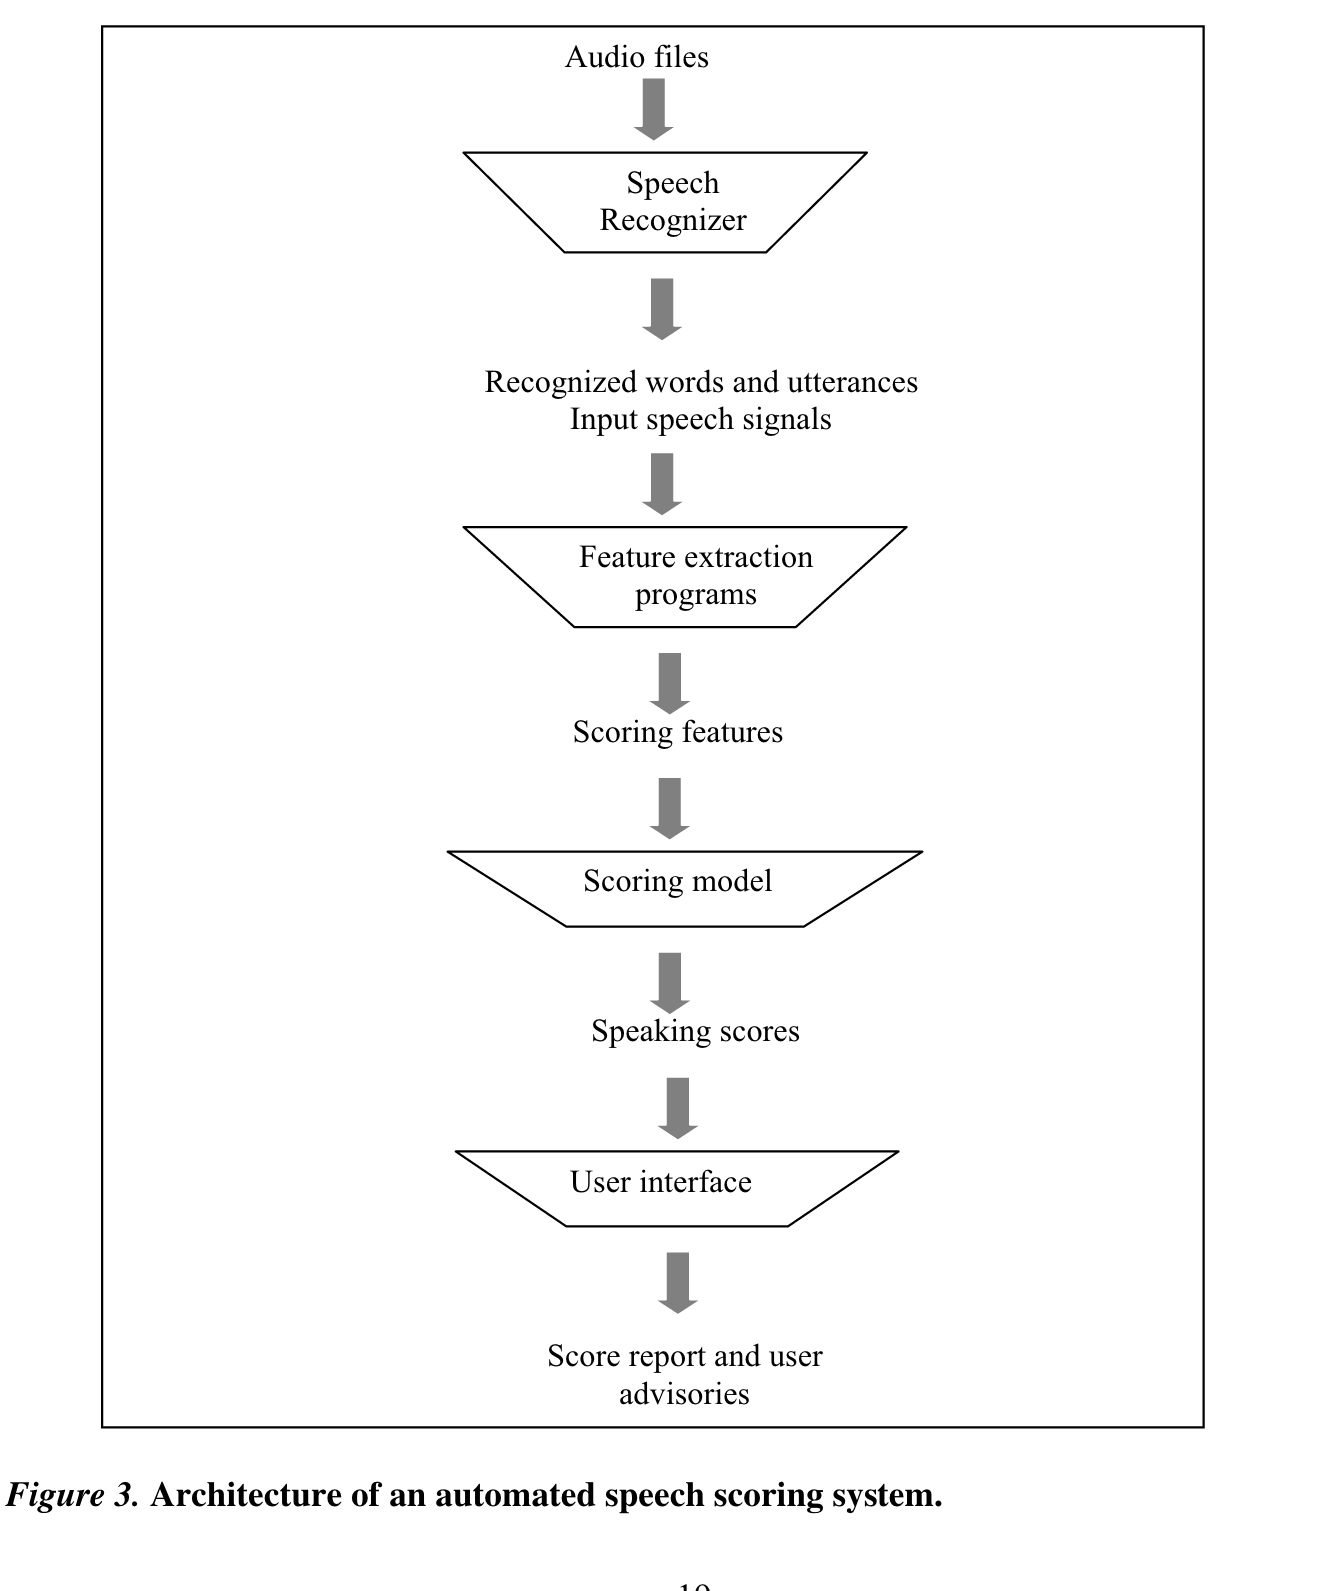
\includegraphics[width=0.6\textwidth]{scoringarch.png}
 \\ \footnotesize source: SpeechRater software by Educational Testing Service
 \\ \url{http://onlinelibrary.wiley.com/doi/10.1002/j.2333-8504.2008.tb02148.x/epdf}
\end{frame}

\begin{frame}
\frametitle{What kind of features should be developed for this task?}
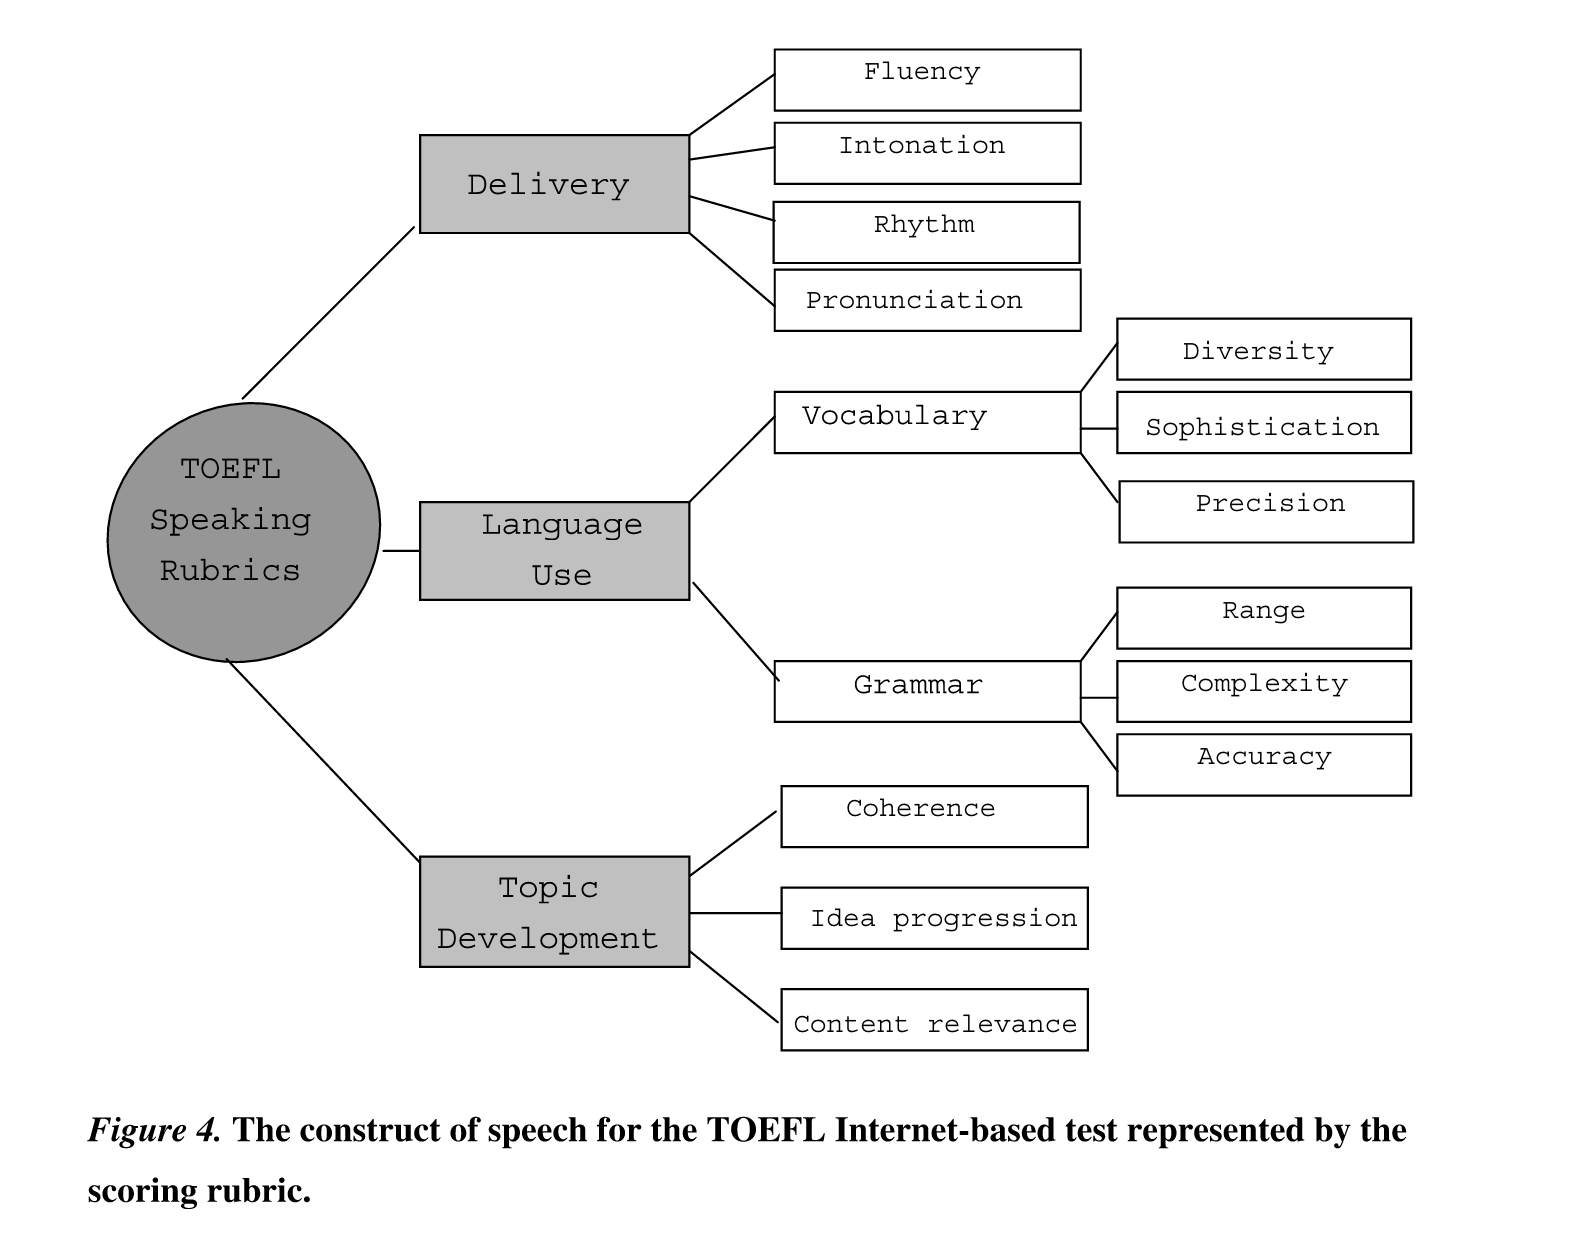
\includegraphics[width=0.8\textwidth]{rubric.png}
 \\ \footnotesize source: SpeechRater technical report from 2008 
 \\ \url{http://onlinelibrary.wiley.com/doi/10.1002/j.2333-8504.2008.tb02148.x/epdf}
\end{frame}

\begin{frame}
\frametitle{Where else speech processing involving language use useful?}
\begin{itemize}
\item Speech based human-computer interfaces (Siri)
\item Speech to Speech translation (Skype translator demo: \url{https://www.youtube.com/watch?v=0I5Is7Qc8yY})
\item Speaker/Dialect identification, detecting deception etc (homeland security)
\item Tutoring systems, voice systems etc. (Hawking's speaker)
\item Studying neuro-generative disorders and others that can affect our use of language (e.g., alzheimers, aphasia, dyslexia etc) (Yes, this is real!)
\end{itemize}
\end{frame}

\begin{frame}
\frametitle{Remaining Weeks}
\begin{itemize}
\item We have three weeks of instruction left (wow!) 
\item There is only one main topic to cover (may be next week): Machine Translation
\item Remaining 2 weeks: Some other assorted topics and discussions, classroom projects, final exam related work.
\item If you want me to discuss something (related to the course!), post on the Canvas forum about discussion topics. 
\item Grade improvement seekers: set up a time to meet in last week of classes, give me any 3 topics you are comfortable with, and do an oral exam with me. (Maximum grade increase: 5\%. If you really do extra-ordinarily well, and if your Assignment scores do not reflect that at all, I can consider increasing further).
\end{itemize}
\end{frame}

\begin{frame}
\frametitle{Final Exam}
\begin{itemize}
\item Carries: 20\% of your grade, and involves writing 2 short essays. 
\item Has to be submitted in three parts:
\begin{enumerate}
\item Write a part of the assignment (one question) and submit by 2nd December - 5\%
\item Do an in-class peer review of one of your classmate's work (6th December) - 5\% - if you don't come to class, you don't get graded for this part.
\item Final submission (of both the questions) - 10\%
\end{enumerate}
\item Exact details about word limits, how to submit and list of topics for questions are on Canvas. 
\end{itemize}
\end{frame}

\begin{frame}
\frametitle{Attendance Exercise}
Our next (last) topic is Machine Translation. Here is a small exercise that will give a preview of what machine translation is. Work in groups of 2--3 people.
\end{frame}

\end{document}
